\documentclass[aps,pra,twocolumn,superscriptaddress,floatfix,longbibliography]{revtex4-2}

\usepackage{amsmath,amssymb}
\usepackage{graphicx}
\usepackage[colorlinks=true,allcolors=blue]{hyperref}

\begin{document}

\title{Relativistic Stark resonances in Debye plasmas: screening undoes
the relativistic suppression of ionization widths}

\author{C.~D.~Reinoso}
\email{cesardanielrrch@gmail.com}
\affiliation{Facultad de Ciencias, Escuela Superior Polit\'ecnica de
Chimborazo (ESPOCH), Riobamba, Ecuador}

\date{\today}

\begin{abstract}
The three ingredients of a hydrogen-like ion in a dense plasma under a
strong static field --- relativity, Debye screening, and field
ionization --- have each been treated in pairs; nonperturbative
resonance parameters of the combined problem have, to our knowledge,
never been reported. We compute them: positions and widths of the
Dirac equation with a Yukawa-screened Coulomb potential and a uniform
electric field, by complex scaling of a coupled $\kappa$-channel
system whose radial channels carry the exact-structure Laguerre bases
of our companion program. The engine is validated on a ladder ---
per-channel Sommerfeld spectra to $10^{-11}$, the relativistic Stark
benchmarks of Maltsev \emph{et al.} to seven digits, and the
nonrelativistic screened-Stark limit against an independent engine to
$4\times10^{-6}$ --- and its spurious $\kappa>0$ intruder, exactly
degenerate with the $1s$ level at zero screening, is identified and
excluded per channel using the pollution theory of our companion
theorem paper. Two results follow. First, in the scaled units
$(\lambda/Z,\,F/Z^{3})$ in which nonrelativistic physics collapses to
a single curve, the relativistic width suppression discovered at zero
screening weakens monotonically as screening grows: the suppression
factor rises by $0.2\%$ at $Z=10$ but by $62\%$ at $Z=82$, so the
plasma catalyzes field ionization of a heavy ion $1.6$ times more
strongly than nonrelativistic scaling predicts --- screening lifts
the level toward threshold and deflates the exponential sensitivity
of the tunneling width to the relativistic binding correction, which
itself survives nearly intact. Second, resolving the $n=2$, $m=1/2$
manifold at $Z=40$ into its three field-dressed components, the
outer pair is born with equal widths where the matched
nonrelativistic doublet is thirty-fold asymmetric, and its width
ratio is non-monotonic in the screening parameter --- falling from
$1.02$ to $0.22$ and recovering to $0.33$ while the nonrelativistic
ratio rises monotonically --- as the uphill component crosses
$E_r=0$ and persists as a positive-energy relativistic resonance.
\end{abstract}

\maketitle

\section{Introduction}

Each pairwise combination of relativity, plasma screening, and static
fields in a hydrogen-like ion is by now classical. The relativistic
Stark problem --- the Dirac equation in a uniform field --- was
solved nonperturbatively by complex rotation for low
$Z$~\cite{IvanovHo2004} and recently mapped across $Z=1$--$82$ by
Maltsev \emph{et al.}~\cite{Maltsev2023}, whose central finding is a
\emph{relativistic suppression} of ionization widths reaching an
order of magnitude at high $Z$. The screened Stark problem at the
nonrelativistic level has a two-decade
lineage~\cite{YuHo2005,LinHo2011,BaharSoylu2014}, extended by our
companion map of the $(F,\lambda)$ plane~\cite{companionD}. The screened Dirac
problem without a field is likewise developed, from bound
levels~\cite{BielinskaWaz2004} to resonances~\cite{Shi2014,
companionB}. The triple combination --- Dirac, screening, and field
at once --- appears never to have been computed at the level of
nonperturbative resonance positions and widths (the three
ingredients do meet in the adjacent line-broadening
literature~\cite{Zenkhri2023,Wu2026}, where the computed quantity is
collisional electron-impact broadening rather than static-field
ionization), although it is the
natural setting for highly charged ions in dense plasmas, and
although the obvious question writes itself: does Maltsev's
relativistic suppression survive when the plasma screens the
Coulomb attraction?

This paper computes the triple and answers the question: the
suppression does not fully survive. Screening lifts the level toward
the continuum threshold; the relativistic deepening of the binding
survives almost intact, but the exponential sensitivity of the
tunneling width to that offset deflates, and the width recovers
toward its nonrelativistic value --- weakly at low $Z$, dramatically
in the heavy-ion regime. In a plasma, a highly charged ion is therefore
doubly fragile: the familiar screening catalysis of field
ionization~\cite{YuHo2005,companionD} is compounded by the removal
of the relativistic width protection.

The tool is a coupled-channel complex-scaling method assembled from
two validated components of our program: the exact-structure radial
Dirac bases (Coulomb--Dirac cusp exponent $r^{\gamma}$, certified
assembly)~\cite{companionA,companionB} and the coupled-channel Stark
machinery of the nonrelativistic companion~\cite{companionD}. The
one genuinely new element --- the relativistic dipole coupling
between $\kappa$-channels --- is certified by two independent
derivations. A known hazard of finite-basis Dirac calculations turns
out to matter operationally: the spurious $\kappa>0$ state that is
\emph{exactly} degenerate with the physical $1s$ level at zero
screening~\cite{DrakeGoldman1981,TupitsynShabaev2008} detaches
downward under screening and, if untreated, silently replaces the
physical reference. Our companion pollution
theory~\cite{companionT} identifies it; per-channel referencing
excludes it by construction.

\section{Method}
\label{sec:method}

\subsection{Coupled $\kappa$-channels}

For a point nucleus of charge $Z$ with Yukawa screening and a field
$F\hat z$ (atomic units, $c=137.035999$),
\begin{equation}
H = c\,\boldsymbol{\alpha}\!\cdot\!\mathbf{p} + \beta c^{2}
    - \frac{Z e^{-\lambda r}}{r} + F z ,
\end{equation}
where $\lambda$ is the inverse Debye length of the plasma, the
magnetic quantum number $m$ is conserved; we work in the lowest
sector $m=1/2$. Each relativistic angular channel, labeled by the
Dirac quantum number $\kappa=\mp(j+\tfrac12)$ for
$j=\ell\pm\tfrac12$ [the eigenvalue of
$-(1+\boldsymbol{\sigma}\cdot\mathbf{L})$],
contributes large and small radial components; the field couples
channels through the angular matrix elements of $\cos\theta$
between spin-angular functions,
$A^{L}_{\kappa'\kappa}=\langle\Omega_{\kappa' m}|\cos\theta|
\Omega_{\kappa m}\rangle$ for the large components and
$A^{S}_{\kappa'\kappa}=A^{L}_{-\kappa',-\kappa}$ for the
small ones, evaluated from the Wigner--Eckart reduced matrix
element~\cite{Grant2007}. These coefficients were certified by an
independent Clebsch--Gordan/Gaunt decomposition, the two derivations
agreeing to machine zero on all pairs; their $s$-limit reproduces
the nonrelativistic Gaunt factor exactly.

Radially, every channel carries the orthonormal exact-structure
Laguerre basis of Ref.~\cite{companionA} ($r^{\gamma_\kappa}$
prefactor, $\gamma_\kappa=\sqrt{\kappa^{2}-(Z/c)^{2}}$) on a
\emph{shared} quadrature grid, so cross-channel dipole integrals
$\langle f_{\kappa'}|r|f_{\kappa}\rangle$ are exact contractions;
production settings use twelve channels
($\kappa=\pm1,\pm2,\dots,\pm6$), $n_b=52$ functions per channel and
component ($2\times52\times12=1248$ degrees of freedom), scale
$\beta=0.55Z$, and
overlap/integration-by-parts certifications at the
$10^{-12}$--$10^{-8}$ level across $Z=1$--$82$. The per-channel
diagonal blocks are the mass-shifted complex-symmetric Dirac pencils
of Ref.~\cite{companionB} under the complex rotation
$r\to re^{i\theta_c}$ (screening evaluated at complex argument),
which exposes each resonance as an isolated complex eigenvalue
$E=E_r-i\Gamma/2$, with $E_r$ the position and $\Gamma$ the full
ionization width; the field blocks are $F e^{i\theta_c}
A^{L,S}_{\kappa'\kappa}\langle f_{\kappa'}|r|f_{\kappa}\rangle$. For
the \emph{nonrelativistic} screened-Stark operator this rotation
rests on dilation-analyticity
theory~\cite{AguilarCombes1971,HerbstSimon1978,Herbst1979}; no
analogous theorem is known for the Dirac operator with a linear
potential, and, as in the relativistic Stark
literature~\cite{IvanovHo2004,Maltsev2023}, complex rotation is
applied here as a computational tool~\cite{Ho1983,Moiseyev1998}
whose operational justification is the two-angle acceptance test and
the validation ladder below.

\subsection{The impostor and its exclusion}

Finite-basis Dirac discretizations of the $\kappa>0$ channels carry
a spurious state exactly degenerate with the physical $1s$
($-\kappa$) level~\cite{DrakeGoldman1981,TupitsynShabaev2008}.
Under screening this degeneracy is lifted the wrong way: the
impostor detaches \emph{downward}, and a full-matrix
lowest-eigenvalue selector then anchors all continuations to an
unphysical, basis-dependent state --- we observed exactly this
failure, flagged because the selected level fell \emph{below} the
variational bound implied by the hydrogenic scaling
$E(Z,\lambda)=Z^{2}E(1,\lambda/Z)$. All field-free references are
therefore taken from the corresponding $\kappa$-channel block alone
(the physical $1s$ from $\kappa=-1$, where no impostor exists),
which excludes the intruder by construction; the mechanism and its
per-fiber theory are the subject of the companion theorem
paper~\cite{companionT}.

\subsection{Identification, scaling, uncertainties}

Resonances are identified as in
Refs.~\cite{companionD,companionB}: parametric continuation (the
search window predicted from the channel-block field-free level plus
the previous complex field shift), two-angle acceptance with the
pairing rule of Ref.~\cite{companionD} and the modulus difference
recorded as the spread. The angle pairs are chosen per $Z$ as the
smallest rotations that expose the resonance while remaining
$\theta$-stable --- the relativistically narrowed high-$Z$
resonances require smaller angles: $\theta_c=0.14/0.22$ at $Z=10$;
$0.10/0.16$ at $Z=20$ and $40$ (including the $n=2$ manifold);
$0.08/0.13$ at $Z=54$ and $82$; the $Z=1$ validation runs used
$0.18/0.26$. We present results in
the scaled variables $u=\lambda/Z$ and $f=F/Z^{3}$, in which
nonrelativistic physics is $Z$-independent
($E=Z^{2}\tilde E$, $\Gamma=Z^{2}\tilde\Gamma$): every deviation
from the collapse is pure relativity. The nonrelativistic baseline
$\tilde\Gamma_{\rm nr}(u,f)$ is computed live with the engine of
Ref.~\cite{companionD}. Quoted uncertainties are two-angle spreads
--- estimates calibrated on the validation ladder, not bounds. The
dominant systematic is channel truncation, calibrated at
$1.4\times10^{-3}$ relative in widths at the production
twelve-channel setting [step~(ii) below], so tabulated suppression
factors are significant to about three digits.

\subsection{Validation ladder}

(i)~Field-free, per channel: exact Dirac--Coulomb (Sommerfeld)
energies reproduced at $10^{-11}$ ($Z\!=\!1$--$40$) to $10^{-8}$
($Z\!=\!92$, $s_{1/2}$). (ii)~Stark, no screening: the benchmarks
of Ref.~\cite{Maltsev2023} at $F/Z^{3}=0.05$ reproduced at
$Z=1,10,18$; at converged settings (20 channels, $n_b=64$) the
$Z=1$ shift agrees to $5\times10^{-8}$ and the width to
$2\times10^{-6}$ relative. (iii)~Screening, low $Z$: at
$Z=1$, $F=0.10$, $\lambda=0.20$ the resonance agrees with the
independently written nonrelativistic engine of
Ref.~\cite{companionD} to $4\times10^{-6}$ --- the residual being
the $1s$ Dirac shift itself. (iv)~The $u=0$ suppression factors
below reproduce the ratios implied by Maltsev's tables (e.g.\
$S=0.4089$ at $Z=54$ versus $0.4088$).

\section{Results}
\label{sec:results}

\subsection{Screening undoes the relativistic width suppression}

Figure~\ref{fig:supp} and Table~\ref{tab:supp} present the central
result: the suppression factor
$S(Z,u)=\Gamma/(Z^{2}\tilde\Gamma_{\rm nr})$ of the $1s$ Stark
resonance at fixed scaled field $f=0.05$, as screening grows from
$u=0$ to $0.20$.

\begin{figure}[tb]
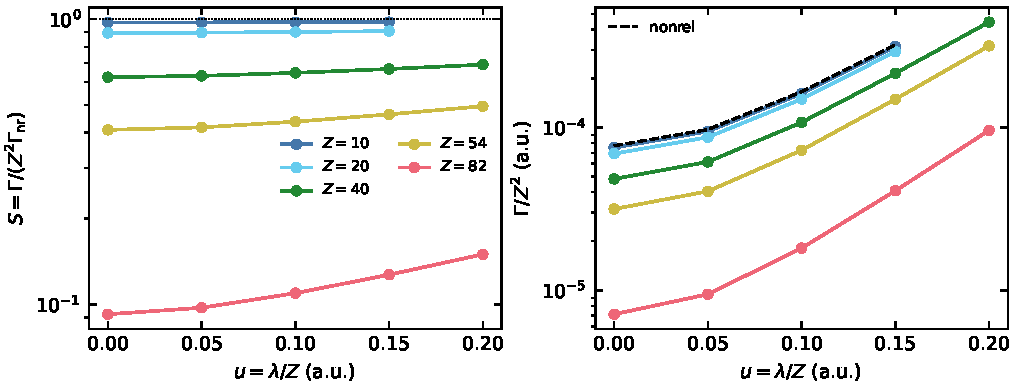
\includegraphics[width=\columnwidth]{figures/figF_suppression}
\caption{\label{fig:supp}Left: relativistic suppression factor
$S=\Gamma/(Z^{2}\Gamma_{\rm nr})$ of the $1s$ Stark resonance at
$f=F/Z^{3}=0.05$ versus scaled screening $u=\lambda/Z$, for
$Z=10$--$82$ (log scale). Screening drives every curve toward the
nonrelativistic limit $S=1$ (dotted). Right: scaled widths
$\Gamma/Z^{2}$; the dashed curve is the nonrelativistic baseline,
on which all $Z$ would collapse in the absence of relativity.}
\end{figure}

\begin{table}[tb]
\caption{\label{tab:supp}Suppression factor $S(Z,u)$ of the $1s$
width at $f=0.05$. Two-angle spreads below $5\times10^{-4}$
(absolute; worst corner $4.4\times10^{-4}$ at $Z=54$, $u=0.20$). The
$u=0$ column reproduces the
field-free-screening ratios implied by Ref.~\cite{Maltsev2023}.}
\begin{ruledtabular}
\begin{tabular}{cccccc}
$Z$ & $u=0$ & $0.05$ & $0.10$ & $0.15$ & $0.20$ \\
\hline
10 & 0.9737 & 0.9740 & 0.9747 & 0.9760 & --- \\
20 & 0.8943 & 0.8963 & 0.9011 & 0.9076 & --- \\
40 & 0.6258 & 0.6324 & 0.6479 & 0.6685 & 0.6924 \\
54 & 0.4089 & 0.4173 & 0.4369 & 0.4635 & 0.4950 \\
82 & 0.0923 & 0.0973 & 0.1094 & 0.1270 & 0.1497 \\
\end{tabular}
\end{ruledtabular}
\end{table}

Every row rises: screening always weakens the relativistic
suppression, and the effect grows steeply with $Z$ --- a $0.2\%$
recovery at $Z=10$, $+10.6\%$ at $Z=40$, $+21\%$ at $Z=54$, and
$+62\%$ at $Z=82$ over the computed range. The mechanism is not an
erosion of the relativistic binding itself: the scaled relativistic
deepening $\Delta(u)=|E_0|/Z^{2}-|E_0^{\rm nr}|$ of the reference
level is nearly independent of screening ($0.0552\to0.0519$ at
$Z=82$; $0.0111\to0.0104$ at $Z=40$), because the Debye potential is
a long-range modification ($e^{-\lambda r}/r\simeq1/r-\lambda$ near
the nucleus) that lifts the level almost uniformly without touching
the short-range relativistic well. What screening deflates is the
exponential lever arm of that offset: semiclassically $\ln S\simeq
-\tfrac{2}{3f}\bigl[(2|E_0|/Z^{2})^{3/2}-(2|E_0^{\rm
nr}|)^{3/2}\bigr]$, and as both levels rise toward threshold the
sensitivity of the tunneling width to the persistent $\Delta$
collapses. This one-line estimate reproduces the data ($S=0.104$
versus the measured $0.0923$ at $Z=82$, $u=0$; $0.175$ versus
$0.1497$ at $u=0.20$), and freezing $\Delta$ at its unscreened value
still yields $S=0.156$ at $u=0.20$: the level lift alone accounts
for roughly $80\%$ of the recovery, the residual outward
displacement of the electron for the rest. The practical statement
compounds with the known screening
catalysis~\cite{YuHo2005,companionD}: at $Z=82$ the absolute width
grows by a factor $13.5$ across the computed screening range,
against $8.3$ for the nonrelativistic catalysis alone --- the
plasma catalyzes field ionization of a heavy ion $1.6$ times more
strongly than nonrelativistic scaling predicts ($13.5/8.3=1.62$,
identically the $62\%$ recovery of $S$), because it simultaneously
deflates the relativistic protection.

\subsection{The $n=2$ manifold: non-monotonic fine-structure
asymmetry}

At $Z=40$ and mild scaled field $f=0.004$ the $m=1/2$, $n=2$
manifold carries three states: the exactly degenerate
$2s_{1/2}$--$2p_{1/2}$ pair and the $2p_{3/2}$, split by the fine
structure ($4.50$ a.u.). An adiabatic field ramp labels the three
field-dressed components by continuation --- the degenerate pair
splits into a downhill component A ($\Delta E=-19.65$, matching the
linear Stark scale) and a central component B, while the
$2p_{3/2}$-dominated C moves uphill ($+13.99$); labels are
continuation labels, not quantum numbers. Screening continuation
then gives the evolution shown in Fig.~\ref{fig:triplet}: the
downhill component's width is catalyzed by a factor
$\sim6000$ across $u\leq0.20$; the uphill component crosses
$E_r=0$ near $u\approx0.19$ and persists as a positive-energy
relativistic resonance, the Dirac analog of the through-threshold
continuations of Refs.~\cite{companionD} (and of the field-free
positive-energy states of Ref.~\cite{companionNR}); the central,
narrowest component dissolves into the mixing beyond
$u=0.05$. The relativistic observable is the width ratio of the
outer pair, for which we computed the matched nonrelativistic
baseline --- the $n=2$, $m=0$ parabolic doublet at the same scaled
field, with the engine of Ref.~\cite{companionD}:
nonrelativistically the uphill/downhill width ratio starts strongly
asymmetric, $\tilde\Gamma_{\rm up}/\tilde\Gamma_{\rm down}=0.031$
at $u=0$, and rises monotonically to $0.22$ by $u=0.15$ (beyond
which the uphill state crosses threshold and its tracking
degrades). The Dirac pair at $Z=40$ resembles this baseline in
neither respect. It is born with \emph{equal} widths
($\Gamma_{\rm C}/\Gamma_{\rm A}=1.02$ at $u=0$): at this $Z$ the
fine-structure splitting is comparable to the Stark coupling, and
the $2p_{3/2}$-dominated component borrows an order of magnitude of
width through spin--orbit mixing. And its ratio is
\emph{non-monotonic}, falling to a minimum of $0.22$ at $u=0.125$
and recovering to $0.33$ by $u=0.20$ --- a five-fold
screening-induced asymmetry that partially heals as both states
approach the continuum.

\begin{figure}[tb]
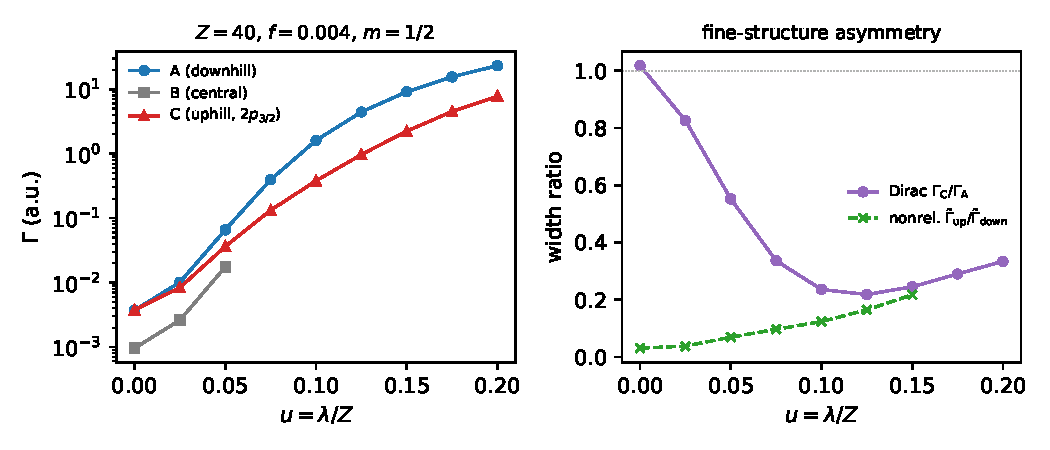
\includegraphics[width=\columnwidth]{figures/figF_triplet}
\caption{\label{fig:triplet}The three field-dressed components of
the $n=2$, $m=1/2$ manifold at $Z=40$, $f=0.004$ under screening.
Left: widths (log scale) of the downhill (A), central (B) and
uphill (C, $2p_{3/2}$-dominated) components. Right: the
fine-structure width ratio $\Gamma_{\rm C}/\Gamma_{\rm A}$ is
non-monotonic in the screening parameter, while the matched
nonrelativistic ratio
$\tilde\Gamma_{\rm up}/\tilde\Gamma_{\rm down}$ (dashed; shown for
$u\leq0.15$, before the nonrelativistic uphill state crosses
threshold) starts thirty-fold asymmetric and rises monotonically.}
\end{figure}

\subsection{Honest limits}

Tracking currently extends to $u=0.15$--$0.20$ at $f=0.05$ (the
broadest states escape the two-angle window; the established trends
are monotonic over $4$--$5$ points per $Z$). At $Z=82$ the
assembly certification degrades to $8\times10^{-8}$ and the $u=0$
width sits $1.4\%$ from Maltsev's value --- the honest error bar of
the extreme-$Z$ row, to be tightened with a basis-convergence
ladder at submission. QED corrections
($\sim\alpha(Z\alpha)^{4}$) and finite nuclear size are neglected
throughout; following Ref.~\cite{Maltsev2023}, all values are
Dirac-level benchmarks. The static Debye potential is the standard
model of this literature~\cite{JanevZhangWang2016}; the
quasistatic-microfield framing of the field follows the companion
discussion~\cite{companionD,Griem1974}.

\section{Conclusions}

The triple problem --- Dirac, Debye screening, static field --- is
computed here, to our knowledge for the first time at the level of
nonperturbative resonance positions and widths, on a validation
ladder that touches every edge of the parameter cube. Its physics
is a two-way coupling that neither pairwise problem contains:
screening does not merely catalyze field ionization, it also erodes
the relativistic suppression of the width, so that at $Z=82$ a
heavy ion in a dense plasma ionizes about $60\%$ faster than the
nonrelativistic and zero-screening treatments combined would
predict; and the fine-structure asymmetry of excited Stark
manifolds is a non-monotonic function of the plasma density where
its nonrelativistic counterpart is monotonic. The spurious-state
exclusion that made the maps possible is itself a working
demonstration of the companion pollution
theory~\cite{companionT}. Extensions within reach of the same
engine include the muonic sector, finite nuclear size, and denser
$(Z,u,f)$ coverage toward line-shape applications. All scripts,
gates and machine-readable maps are distributed with the companion
programs and will be archived with a persistent identifier at
publication.

\begin{acknowledgments}
The author thanks the ESPOCH Faculty of Sciences for institutional
support.
\end{acknowledgments}

\bibliography{refs}

\end{document}
